% JETSPIN structure documentation

\section{Structure\label{sec:Structure}}

JETSPIN is written in free format FORTRAN90, and it consists of approximately
160 subroutines. The source exploits the modular approach provided
by the programming language. All the variables having in common description
of certain features or method are grouped in modules. The convention
of explicit type declaration is adopted, and all the arguments passed
in calling sequences of functions or subroutines have defined intent.
We use the PRIVATE and PUBLIC accessibility attributes in order to
decrease error-proneness in programming.

The main routines have been gathered in the \texttt{main.f90} file,
which drives all the CPU-intensive computations needed for the capabilities
mentioned below. The variables describing the main features of nanofibers
(position, velocity, etc.) are declared in the \texttt{nanojet\_mod.f90}
file, which also contains the main subroutines for the memory management
of the fundamental data of the simulated system. Since the size system
is strictly time-dependent, JETSPIN exploits the dynamic array allocation
features of FORTRAN90 to assign the necessary array dimensions. In
particular, the size system is modified by the routines \texttt{add\_jetbead}
and \texttt{erase\_jetbead}, while the decision of the main array
size, declared as \texttt{mxnpjet}, is handled by the routine \texttt{reallocate\_jet}.
The sizes of various service bookkeeping arrays are handled within
a parallel implementation strategy, witch exploits few dedicated subroutines
(see Sec \ref{sec:Parallelization}). All the implemented time integrators
are written in the \texttt{integrator\_mod.f90} file, which contains
the routine \texttt{driver\_integrator} to select the proper integrator,
as indicated in the input file. All the terms of equations of motion
for the implemented model (see Sec \ref{sec:Equation-of-Motion})
are computed by routines located in the \texttt{eom\_mod.f90} file,
which call other subroutines in the files \texttt{coulomb\_force\_mod.f90},
\texttt{viscoelastic\_force\_mod.f90} and \texttt{support\_functions\_mod.f90}.
A summarizing scheme of the main JETSPIN program in the \texttt{main.f90}
file has been sketched in Fig \ref{Fig:Structure-program}.

The user can carry out simulations of nanofibers without a detailed
understanding of the structure of JETSPIN code. All the parameters
governing the system can be defined in the input file (see Sec \ref{sec:Input-file}),
which is read by routines located in the \texttt{io\_mod.f90} and
\texttt{parse\_mod.f90} files. Instead, the user should be acquainted
with the model described in Cap \ref{chap:JETSPIN-Model-and}. The
content of the output file is completely customizable by the input
file as described in Sec \ref{sec:Input-file}, and it can report
different time-averaged observables computed by routines of the module
\texttt{statistic\_mod} (see Sec \ref{sec:Output-files}). The routines
in the \texttt{error\_mod.f90} file can display various warning or
error banners on computer terminal, so that the user can easily correct
the most common mistakes in the input file.

JETSPIN is supplied as a single UNIX compressed (tarred and gzipped)
directory with four sub-directories. All the source code files are
contained in the \textit{source} sub-directory. The \textit{examples}
sub-directory contains different test cases that can help the user
to edit new input files. The \textit{build} sub-directory stores a
UNIX \texttt{makefile} that assembles the executable versions of the
code both in serial and parallel versions with different compilers.
It is invoked from the repository root while using the \textit{source}
sub-directory as its working directory (see Section
\ref{sec:Compiling-the-Source}); it does not need to be copied.
Finally, after JETSPIN was compiled, the \textit{execute} sub-directory
contains the binary executable file, where it can be run.

\begin{figure}
\begin{centering}
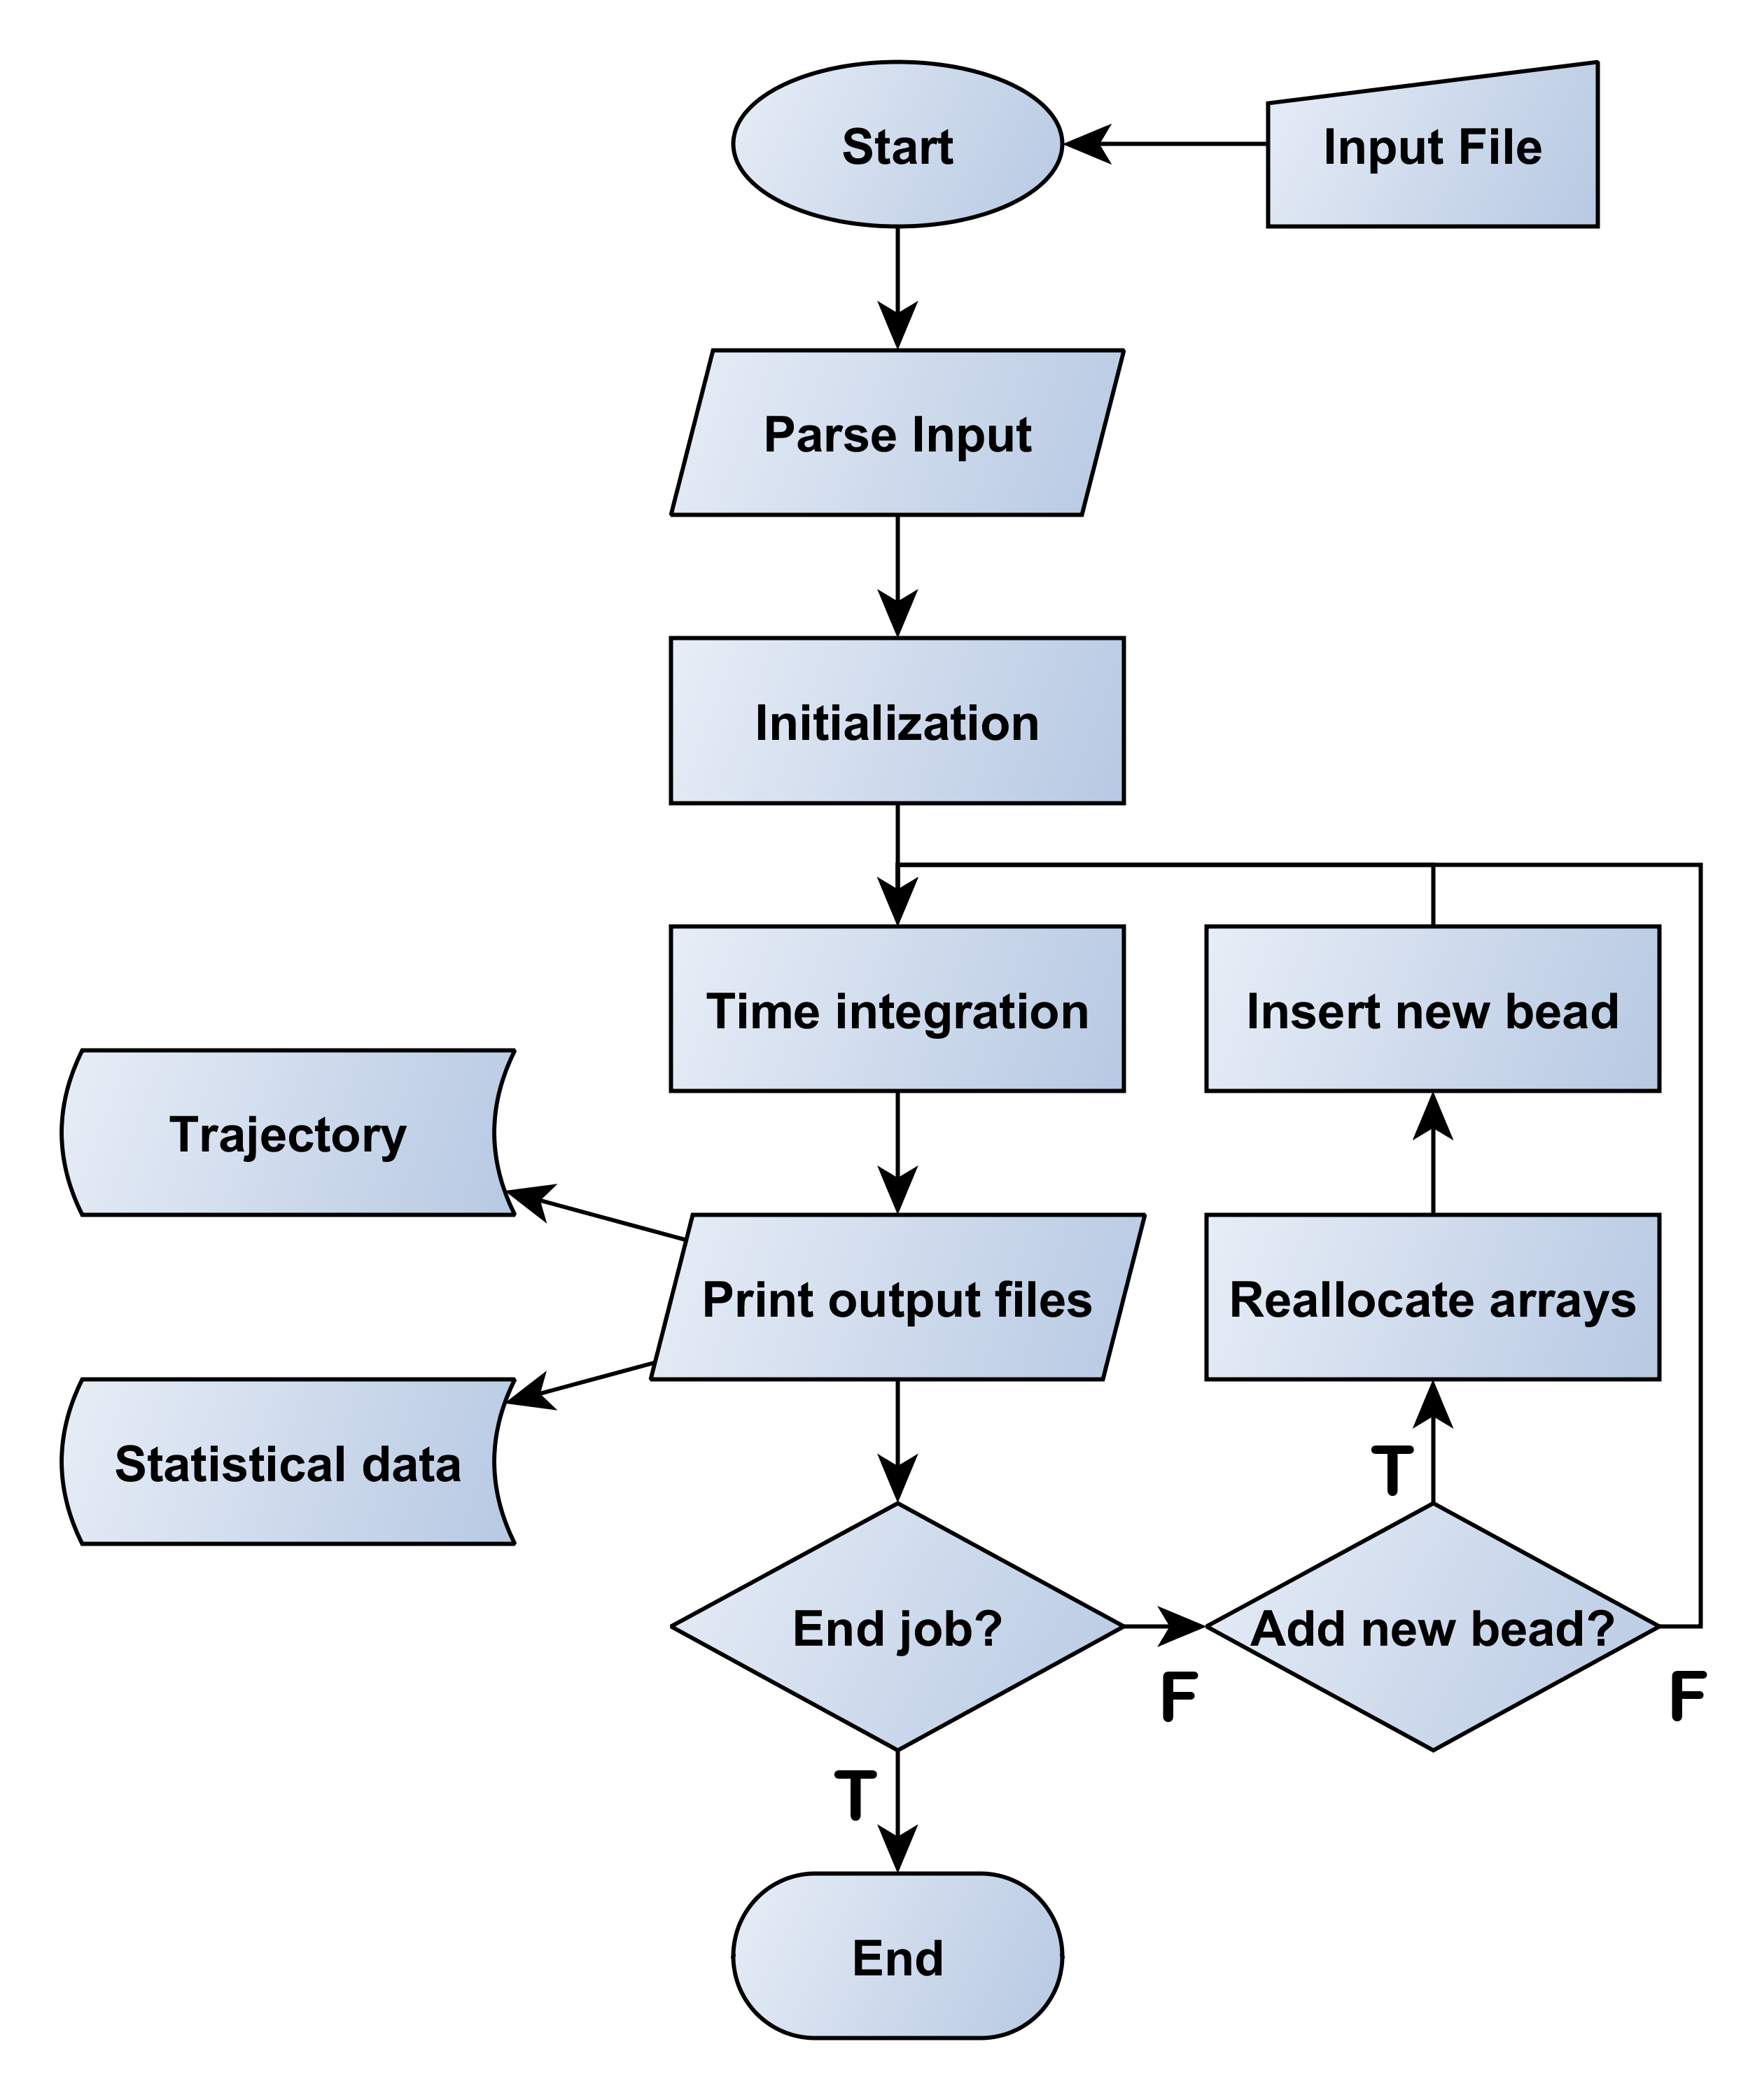
\includegraphics[scale=0.18]{figure01}
\par\end{centering}
\protect\caption{Structure of the main JETSPIN program.}

\label{Fig:Structure-program}
\end{figure}
